\documentclass[10pt,twocolumn]{article}

\usepackage[utf8]{inputenc}
\usepackage[T1]{fontenc}
\usepackage{lmodern}
\usepackage[protrusion=true,expansion=false]{microtype}
\usepackage[a4paper, top=1.9cm, bottom=1.9cm, left=1.65cm, right=1.65cm, columnsep=0.65cm]{geometry}
\usepackage{amsmath, amssymb, amsfonts, amsthm}
\usepackage{graphicx}
\usepackage{booktabs}
\usepackage{xcolor}
\usepackage{hyperref}
\usepackage{enumitem}

\definecolor{linkblue}{RGB}{20, 70, 140}
\hypersetup{
    colorlinks=true,
    linkcolor=linkblue,
    citecolor=linkblue,
    urlcolor=linkblue,
    pdftitle={HySA: Hybrid Semantic Architecture},
    pdfauthor={Francesco Mariani}
}

\newtheorem{proposition}{Proposition}
\theoremstyle{definition}
\newtheorem{definition}{Definition}

\title{\vspace{-1.0cm}\textbf{\Large HySA (Hybrid Semantic Architecture): Preserving Polysemantic Abstraction via Contrastive Inference Tensors, Monosemantic Indexing, and Topological Temperature \texorpdfstring{($T_t$)}{(Tt)}}}

\author{
    \textbf{Francesco Mariani} \\
    \textit{Independent Systems Architect} \\
    Umbria, Italy \\
    \texttt{fratorials@gmail.com} \\
    {\footnotesize DOI: \href{https://doi.org/10.5281/zenodo.23456159}{\texttt{10.5281/zenodo.23456159}}}
}

\date{October 2026}

\begin{document}

\twocolumn[
  \begin{@twocolumnfalse}
    \maketitle
    \begin{center}
        \vspace{-0.35cm}
        \textit{``The AI industry views polysemanticity as a curse... yet perhaps it is the very blessing that made intelligence possible.''}
        \vspace{0.25cm}
    \end{center}
    \begin{abstract}
      \noindent Contemporary \textit{Mechanistic Interpretability} research predominantly treats neuronal polysemanticity as an undesirable artifact of dimensional compression (\textit{the Superposition Hypothesis}), focusing on decomposing latent spaces into vast, sparse dictionaries of purely monosemantic features. In this work, we propose a paradigm shift: \textbf{polysemanticity is not a defect to be eradicated, but the geometric prerequisite for intelligence and analogical reasoning.} A purely monosemantic neuron is intrinsically ``stupid'' ($\emptyset$ intelligence): lacking cross-domain associative connections, it functions as a rigorous yet sterile memory cell. To decouple fluid associative behavior from deterministic factual verification without resorting to serial architectures (which introduce non-abstractive bottlenecks) or parallel networks (which are computationally inefficient), we introduce \textbf{HySA (\textit{Hybrid Semantic Architecture})}, a unified paradigm delimited by neuronal semanticity. HySA introduces four core contributions: (1) \textbf{Contrastive Inference Superposition} ($I_n$), extracting the multi-concept cube of polysemantic units via weighted inference expectations over contrastive datasets; (2) \textbf{Monosemantic Indexing}, coupling a polysemantic network ($N_p$, intelligence) with an indexed registry of monosemantic centroids ($N_m / N_k$, memory) queried via deterministic internal APIs; (3) the \textbf{Semantic Hypersphere}, governed by dual temperatures ($T_p, T_m$) and \textbf{Topological Temperature} ($T_t$); and (4) the \textbf{Compression Gradient} ($\Delta q$) between $N_p$ and $N_m$, governed by the Degree of Determinism $\beta = T/q$ around a stationary \textbf{Critical Point} ($P_c$).
      \vspace{0.35cm}
    \end{abstract}
  \end{@twocolumnfalse}
]

\section{Introduction: Intelligence vs. Memory}
In deep neural networks, individual units consistently exhibit \textit{mixed selectivity}~\cite{rigotti2013importance, elhage2022toy}. Prevailing approaches utilizing \textit{Sparse Autoencoders} (SAEs)~\cite{bricken2023monosemanticity, templeton2024scaling} seek to disentangle these representations into orthogonal, monosemantic dimensions. However, this pursuit of pure monosemanticity overlooks a fundamental epistemological division between \textbf{Intelligence} and \textbf{Memory}:
\begin{itemize}[leftmargin=*, itemsep=1.5pt, topsep=2pt]
    \item \textbf{Polysemantic Neurons} ($N_p$) \textbf{Generate Intelligence:} A unit co-activating across concepts such as \texttt{IP}, \texttt{DNS}, \texttt{White Pages}, and \texttt{Phone Number} is not experiencing noisy interference. It is compressing multiple concepts into a unified higher-order meaning: the relational schema of \textit{identity-to-address resolution}. \textbf{Associative connections are what make a system intelligent.}
    \item \textbf{Monosemantic Neurons} ($N_m$) \textbf{Provide Memory:} Units encoding rigid atomic literals---such as the IP address \texttt{8.8.8.8}, the integer \texttt{24}, or the proper noun \texttt{JOHN}---possess zero associative connections ($\emptyset$ intelligence). Like entries in a static dictionary, a monosemantic unit is cognitively ``stupid,'' yet it is \textbf{strictly rigorous}---making it essential for preventing hallucinations.
\end{itemize}

Modern LLMs hallucinate because they entangle both regimes within homogeneous weight matrices~\cite{geva2021transformer}, allowing associative gradients to interpolate across immutable facts.

\begin{figure*}[t]
    \centering
    \IfFileExists{fig1_imprinted_tensors.pdf}{
        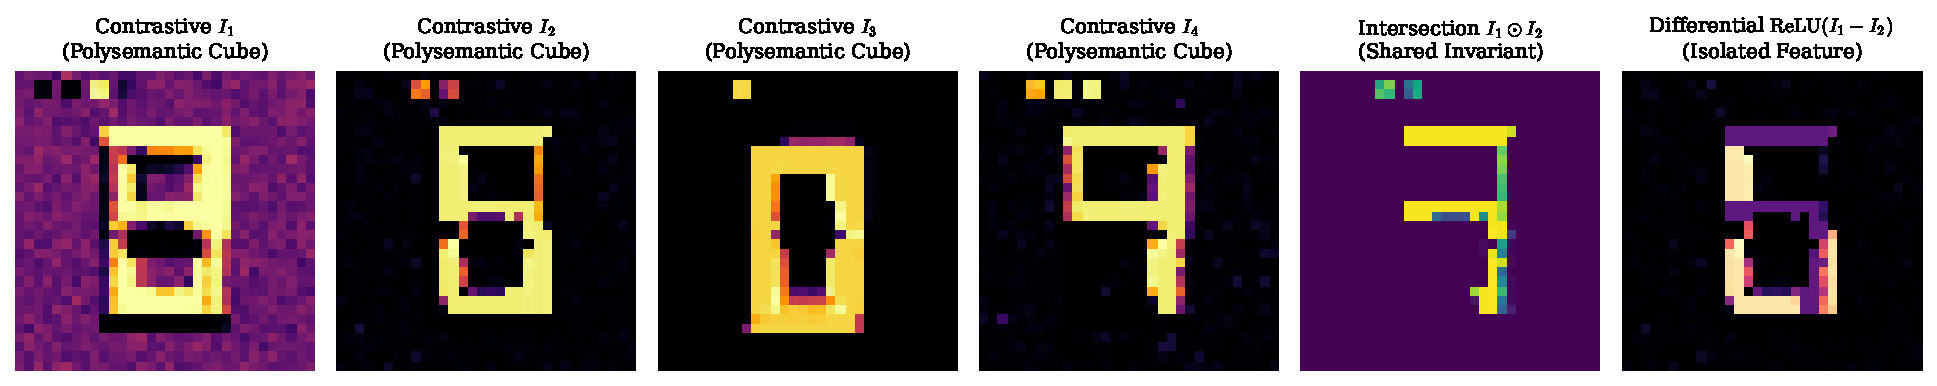
\includegraphics[width=0.98\textwidth]{fig1_imprinted_tensors.pdf}
    }{
        \fbox{\parbox{0.95\textwidth}{\centering \vspace{0.8cm} \textbf{[Figure 1]} \vspace{0.8cm}}}
    }
    \vspace{-0.15cm}
    \caption{\textbf{Contrastive Superposition Tensors ($I_n$) and Algebraic Semantic Queries on the $32 \times 32$ Benchmark.} Columns 1--4 show polysemantic representations learned by a 4-neuron bottleneck. Column 5 isolates the shared invariant ($I_1 \odot I_2$). Column 6 extracts differential feature divergence ($\mathrm{ReLU}(I_1 - I_2)$).}
    \label{fig:imprinted_tensors}
\end{figure*}

\section{Clarification of Systems Terminology}
Each indexed unit $N_k$ possesses a monosemantic centroid $\mu_k$ structurally analogous to an operating system \textbf{``Inode''}, which motivates our use of the term \textbf{``Filesystem''}. To prevent cross-disciplinary ambiguity, Table~\ref{tab:terminology} maps these systems heuristics to their formal mathematical constructs in latent space $\mathcal{S} \subset \mathbb{R}^D$.

\begin{table}[h]
\centering
\caption{Mapping Systems Heuristics to Formal Constructs.}
\label{tab:terminology}
\vspace{0.15cm}
\scriptsize
\begin{tabular}{@{}p{1.9cm}p{2.3cm}p{3.0cm}@{}}
\toprule
\textbf{Systems Term} & \textbf{Formal Construct} & \textbf{Architectural Role} \\ \midrule
\textbf{``Inode''} ($N_k$) & Centroid $\mu_k \in \mathbb{R}^D$ & Orthogonal pointer to an immutable atomic literal (e.g., \texttt{8.8.8.8}). \\[3pt]
\textbf{``Filesystem''} & Indexed Manifold $\mathcal{F}_{\mathrm{mono}} = \{\mu_1, \dots, \mu_M\}$ & Dictionary storage ($\emptyset$ intelligence, $100\%$ rigor) for verification. \\[3pt]
\textbf{``Query / API''} & Metric Operator $Q(q, \mathcal{F}_{\mathrm{mono}}, T_t)$ & Deterministic boundary check confirming polysemantic states. \\ \bottomrule
\end{tabular}
\end{table}

\section{Contrastive Superposition Tensors \texorpdfstring{($I_n$)}{(In)}}
A polysemantic neuron functions as a high-dimensional superposition cube compressing multiple concepts into unified meanings. Because an isolated neuron is a mute scalar, its internal geometry is extracted as the \textbf{weighted average of all inference outputs across a contrastive dataset} ($\mathcal{X}^+$ containing shared structural invariants vs. $\mathcal{X}^-$ baseline):
\begin{equation}
\begin{aligned}
    I_n = \frac{1}{\sum_{k} z_{k,n} + \eta} \bigg[ & \sum_{X_k \in \mathcal{X}^+} z_{k,n} \cdot \Phi_{\mathrm{net}}(X_k \mid n) \\
    & - \gamma \sum_{X_j \in \mathcal{X}^-} z_{j,n} \cdot \Phi_{\mathrm{net}}(X_j \mid n) \bigg]
\end{aligned}
\label{eq:imprinted_tensor}
\end{equation}
where $z_{k,n}$ is unit $n$'s activation and $\Phi_{\mathrm{net}}(\cdot \mid n)$ is the whole-network inference conditioned on $n$. Shared invariants are queried via $I_A \odot I_B$ and divergences via $\mathrm{ReLU}(I_A - I_B)$ (Figure~\ref{fig:imprinted_tensors}).

\section{The Unified Hybrid Paradigm (HySA)}
How should polysemantic intelligence ($N_p$) and monosemantic memory ($N_m$) interact?
\begin{itemize}[leftmargin=*, itemsep=1.5pt, topsep=2pt]
    \item \textbf{Neither Serial:} Placing a rigid monosemantic layer downstream of $N_p$ creates a \textit{non-abstractive bottleneck} that destroys contextual relations.
    \item \textbf{Nor Parallel:} Executing duplicate networks concurrently is \textit{extremely inefficient} computationally.
\end{itemize}
In \textbf{HySA}, the model is a \textbf{unified whole}, delimited internally by logic and by the specific ``semanticity'' (dimensionality and cardinality $M$) of individual neurons within the layers. Fluid reasoning propagates through $N_p$; when factual confirmation is required, the trajectory executes a concise internal \textbf{Query/API} to the indexed monosemantic centroids $\mathcal{F}_{\mathrm{mono}}$, imparting deterministic consistency.

\begin{figure*}[t]
    \centering
    \IfFileExists{fig2_phase_transition.pdf}{
        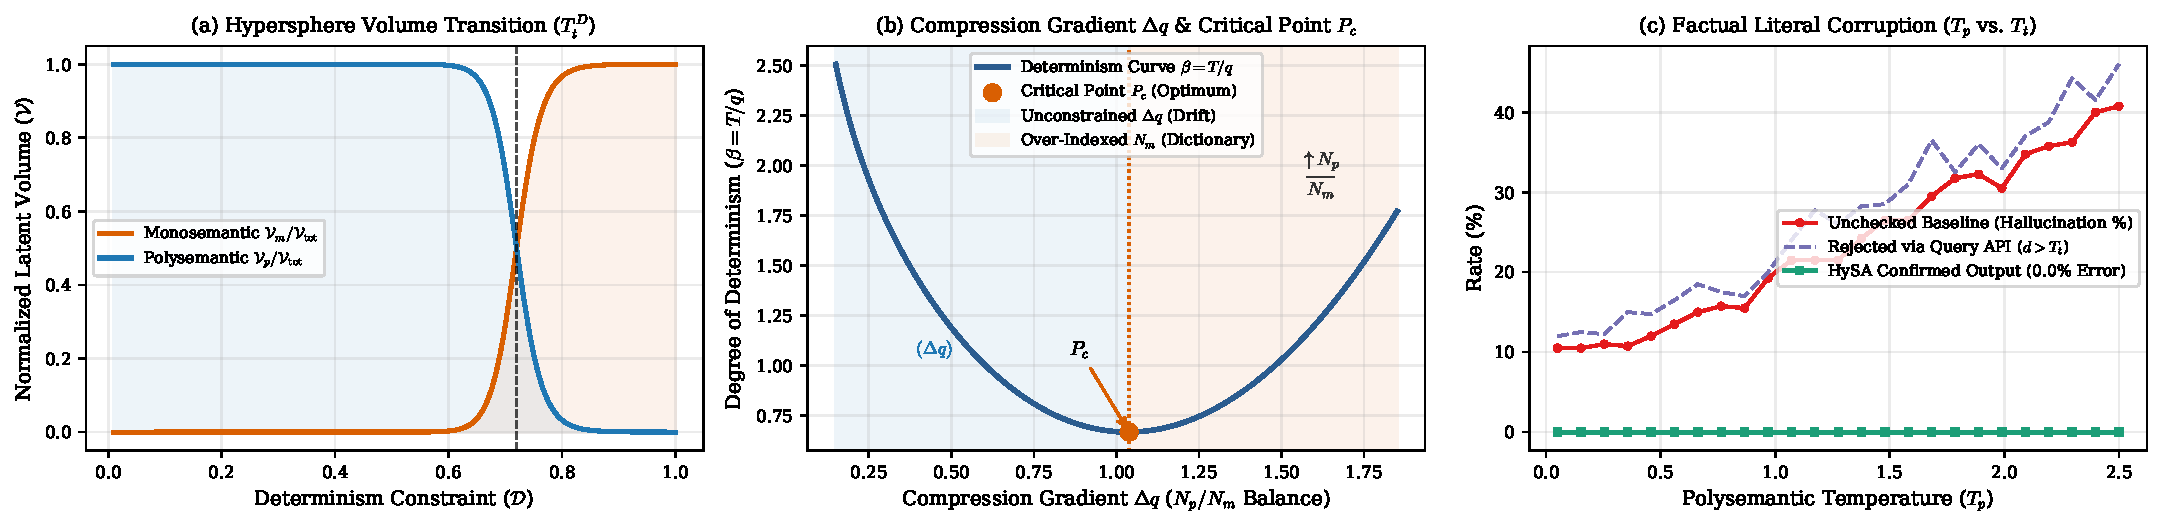
\includegraphics[width=0.98\textwidth]{fig2_phase_transition.pdf}
    }{
        \fbox{\parbox{0.95\textwidth}{\centering \vspace{0.8cm} \textbf{[Figure 2]} \vspace{0.8cm}}}
    }
    \vspace{-0.15cm}
    \caption{\textbf{High-Dimensional Volume Phase Transition, Critical Point ($P_c$), and Factual Verification in HySA.} \textbf{(a)} Step-function transition between Free Polysemantic Volume $\mathcal{V}_p$ and Monosemantic Constraint Volume $\mathcal{V}_m$. \textbf{(b)} Compression gradient $\Delta q$ potential curve displaying the stationary Critical Point $P_c$ over $\beta = T/q$. \textbf{(c)} Unchecked decoding suffers climbing factual corruption, whereas HySA maintains $0.0\%$ corruption via monosemantic API confirmation within $T_t$.}
    \label{fig:phase_transition}
\end{figure*}

\section{The Semantic Hypersphere and Dual Temperatures \texorpdfstring{($T_p, T_m, T_t$)}{(Tp, Tm, Tt)}}
Rather than applying temperature as post-hoc \textit{Softmax} noise, HySA defines temperature geometrically as \textbf{the multidimensional neighborhood of the neuron}: a \textbf{Semantic Hypersphere} in latent space.

When a latent trajectory is \textit{queried} within this hypersphere (where related tokens or concepts such as \texttt{CAT}, \texttt{GATTO}, \texttt{KG}, or \texttt{MACCHINA} lie along radial vectors $A, B, C, D$), system dynamics are governed by two regime temperatures---the \textbf{Polysemantic Temperature} ($T_p$) and \textbf{Monosemantic Temperature} ($T_m$)---bounded by the \textbf{Topological Temperature} ($T_t$):
\begin{equation}
    B(\mu_k, T_t) = \left\{ x \in \mathcal{S} \;\middle|\; \| x - \mu_k \|_2 \le T_t(T_p, T_m) \right\}
\end{equation}
If a queried point $q$ falls within radius $T_t$ of centroid $\mu_k$, the API confirms the reasoning step and binds the exact literal from $\mu_k$. If $\|q - \mu_k\|_2 > T_t$, HySA raises a deterministic \textit{Semantic Fault}, halting hallucination (Figure~\ref{fig:phase_transition}).

\section{Compression Gradient \texorpdfstring{($\Delta q$)}{(Delta q)}, Determinism \texorpdfstring{($\beta$)}{(beta)}, and Critical Point \texorpdfstring{($P_c$)}{(Pc)}}
The structural ratio between polysemantic neurons ($N_p$) and monosemantic centroids ($N_m$) defines the \textbf{Compression Gradient} ($\Delta q$) across layers. Let $q = f(N_p, N_m, M)$ represent the effective neuronal quantity. We define the \textbf{Degree of Determinism} ($\beta$) as:
\begin{equation}
    \beta = \frac{T}{q}
\end{equation}
Mapping $\beta$ against the compression gradient $\Delta q$ yields a convex potential landscape with a stationary minimum at the \textbf{Critical Point} ($P_c$, Figure~\ref{fig:phase_transition}b):
\begin{enumerate}[leftmargin=*, itemsep=1.5pt, topsep=2pt]
    \item \textbf{Left of $P_c$ (Under-Constrained $\Delta q$):} Dominance of $N_p$ without sufficient $N_m$ indexing leads to ungrounded associative drift.
    \item \textbf{Right of $P_c$ (Over-Indexed Saturation):} Dominance of $N_m$ severs associative links; $\mathcal{V}_m \propto M \cdot (T_t)^D$ saturates the space, freezing the model into a static dictionary.
    \item \textbf{At the Critical Point ($P_c$):} Optimal equilibrium between $N_p$ and $N_m$, maximizing polysemantic abstraction while guaranteeing deterministic verification.
\end{enumerate}

\section{Experimental Validation}
We validate HySA across two complementary benchmarks:
\begin{enumerate}[leftmargin=*, itemsep=1.5pt, topsep=2pt]
    \item \textbf{$32 \times 32$ Contrastive Benchmark:} A 4-neuron bottleneck trained on dual-nature binary matrices (shared digit loops + rigid 2$\times$2 top-left literal checksums). As shown in Figure~\ref{fig:imprinted_tensors} and Figure~\ref{fig:phase_transition}c, algebraic queries ($I_1 \odot I_2$ and $\mathrm{ReLU}(I_1 - I_2)$) isolate structural invariants, while the Query API maintains \textbf{$0.0\%$ factual literal corruption} across $T_p \in [0.05, 2.5]$.
    \item \textbf{Real-World Transformer Validation (\texttt{Pythia-70M}):} Probing Layer 3 residual streams ($D=512$) on \texttt{EleutherAI/pythia-70m} confirms that isomorphic concepts (\texttt{DNS}, \texttt{IP Routing}, \texttt{White Pages}, \texttt{Phone Directory}) converge onto a shared polysemantic subspace with cosine similarities between $\mathbf{0.893}$ and $\mathbf{0.973}$ (Table~\ref{tab:pythia}). Indexing normalized monosemantic centroids ($N_k$) on $S^{511}$ with radius $T_t = 0.46$ successfully confirms valid queries (\texttt{8.8.8.8}, \texttt{24}, \texttt{JOHN}, ports \texttt{22}/\texttt{80}, with $d \in [0.089, 0.430] \le T_t$) while intercepting unverified subterranean telemetry queries via a deterministic \textit{Semantic Fault} ($d = 0.497 > T_t$).
\end{enumerate}

\begin{table}[h]
\centering
\caption{Layer 3 Cosine Similarity of Isomorphic Concepts in $N_p$ (\texttt{Pythia-70M}, $D=512$).}
\label{tab:pythia}
\vspace{0.1cm}
\scriptsize
\begin{tabular}{@{}lcccc@{}}
\toprule
\textbf{Concept in $N_p$} & \textbf{DNS} & \textbf{IP Routing} & \textbf{White Pages} & \textbf{Phone Dir.} \\ \midrule
\textbf{DNS} & $1.000$ & $0.961$ & $0.973$ & $0.893$ \\
\textbf{IP Routing} & $0.961$ & $1.000$ & $0.940$ & $0.916$ \\
\textbf{White Pages} & $0.973$ & $0.940$ & $1.000$ & $0.903$ \\
\textbf{Phone Dir.} & $0.893$ & $0.916$ & $0.903$ & $1.000$ \\ \bottomrule
\end{tabular}
\end{table}

\section{Conclusion}
\textbf{HySA} demonstrates that polysemanticity is the core engine of neural intelligence ($N_p$), while monosemanticity is the rigorous guardian of factual memory ($N_m$). By coupling both regimes within a unified architecture governed by the Semantic Hypersphere ($T_t$) at the Critical Point ($P_c$), models achieve creative generalization with deterministic factual consistency.

\begin{thebibliography}{9}
\footnotesize
\bibitem{rigotti2013importance} M.~Rigotti \textit{et al.}, ``The importance of mixed selectivity in complex cognitive tasks,'' \textit{Nature}, vol.~497, pp.~585--590, 2013.
\bibitem{elhage2022toy} N.~Elhage \textit{et al.}, ``Toy models of superposition,'' \textit{Transformer Circuits Thread}, 2022.
\bibitem{bricken2023monosemanticity} T.~Bricken \textit{et al.}, ``Towards monosemanticity: Decomposing language models with dictionary learning,'' \textit{Transformer Circuits Thread}, 2023.
\bibitem{templeton2024scaling} A.~Templeton \textit{et al.}, ``Scaling monosemanticity: Extracting interpretable features from Claude 3 Sonnet,'' \textit{Transformer Circuits Thread}, 2024.
\bibitem{geva2021transformer} M.~Geva \textit{et al.}, ``Transformer feed-forward layers are key-value memories,'' in \textit{Proc. EMNLP}, pp.~5484--5495, 2021.
\end{thebibliography}

\end{document}